\documentclass{beamer} % [aspectratio=169]
\usetheme{ucl}
\setbeamercolor{banner}{bg=darkred}
\setbeamersize{description width=2em}
\setbeamertemplate{navigation symbols}{\vspace{-2ex}} 
\usepackage{soul}

%\usepackage{fontspec}Hash
\usepackage[utf8]{inputenc}
% \usepackage[english, greek]{babel}


\usepackage[T1]{fontenc} % Turn £ into $
\usepackage{minted}
\usemintedstyle{emacs}

\usepackage{fancyvrb}
\usepackage{xcolor}
\usepackage{url}

\usepackage{natbib}
\usepackage{bibentry}
\usepackage{url}
\usepackage{amsfonts}


\usepackage{tikz}
\usetikzlibrary{positioning}
\usetikzlibrary{calc,shapes.multipart,chains,arrows}
\usetikzlibrary{shapes,snakes}

\tikzset{
  treenode/.style = {align=center, inner sep=0pt, text centered,
    font=\sffamily},
  arn_n/.style = {treenode, circle, draw=black,
     text width=1.5em},% arbre rouge noir, noeud noir
  arn_r/.style = {treenode, circle, red, draw=red, 
    text width=1.5em, very thick},% arbre rouge noir, noeud rouge
  arn_d/.style = {treenode, star, star points=10, red, draw=red, 
    text width=1.5em, very thick},% arbre rouge noir, noeud rouge
  arn_x/.style = {treenode, rectangle, draw=black}% arbre rouge noir, nil
}

\newcommand\emc[1]{\textcolor{midred}{\textbf{#1}}}
\newcommand\good[1]{\textcolor{darkgreen}{\textbf{#1}}}
\newcommand\bad[1]{\textcolor{red}{\textbf{#1}}}

\AtBeginSection[]{
  \begin{frame}
  \vfill
  \centering
  \begin{beamercolorbox}[sep=8pt,center,shadow=true,rounded=true]{title}
    \usebeamerfont{title}\insertsectionhead\par%
  \end{beamercolorbox}
  \vfill
  \end{frame}
}

\author{Mark Handley, University College London, UK}
\title{Dynamic Data Structures: Hash Tables\\Algorithms: Searching}
\subtitle{ENGF0002: Design and Professional Skills }
% \institute{}
\date{Term 1, 2019}


\begin{document}
\nobibliography*


\frame{
\titlepage
}

\begin{frame}
\frametitle{The builtin \texttt{dict} type.}

The Python dictionary type provides a very efficient key-value store.
\begin{itemize}
  \item the \texttt{dict} function takes a sequence of tuples and returns a dictionary mapping them as key values.
  \item There is a shorthand for dict literals, eg. \texttt{\{k1:v1, k2:v2\}}
  \item Get and set operations are as in minimap, eg. \texttt{m[k] = v} for set, and \texttt{m[k]} for get.
  \item the \texttt{len} function returns the number of items, and an iterator returns an unordered sequence of keys.
\end{itemize}

\vspace{3mm} 
For a full list of operations see \url{https://docs.python.org/3.7/library/stdtypes.html\#mapping-types-dict}.
\end{frame}

\begin{frame}
\frametitle{Python \texttt{dict} example}
  
\inputminted[
    firstline=2,
    lastline=13,
    xleftmargin=1.4em,
    %frame=lines,
    %framesep=2mm,
    baselinestretch=1.2,
    bgcolor=stone,
    fontsize=\scriptsize,
    linenos
  ]{python}{src/dict.py}
\end{frame}

\begin{frame}
\frametitle{Dict of Dicts}
  
\inputminted[
    firstline=2,
    lastline=11,
    xleftmargin=1.4em,
    %frame=lines,
    %framesep=2mm,
    baselinestretch=1.2,
    bgcolor=stone,
    fontsize=\scriptsize,
    linenos
  ]{python}{src/dict2.py}
\end{frame}


\section{Search}

\begin{frame}
  \centering
  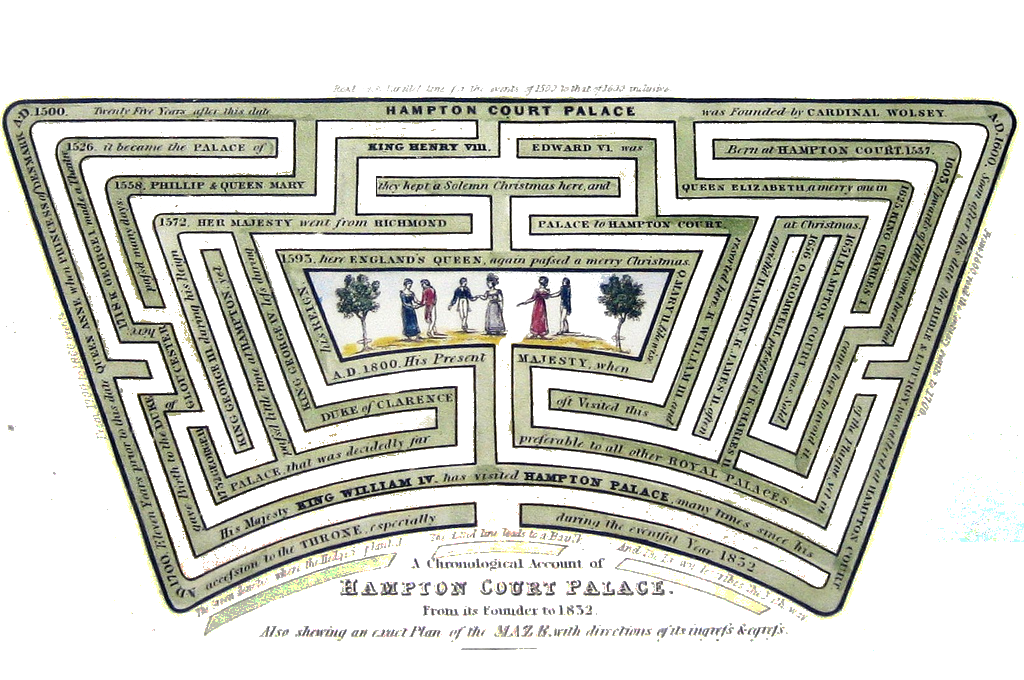
\includegraphics[height=80mm]{assets/hampton1.png}
\end{frame}

\begin{frame}
  \centering
  
\includegraphics[height=50mm]{assets/maze.pdf}
\end{frame}

\begin{frame}
  \centering
  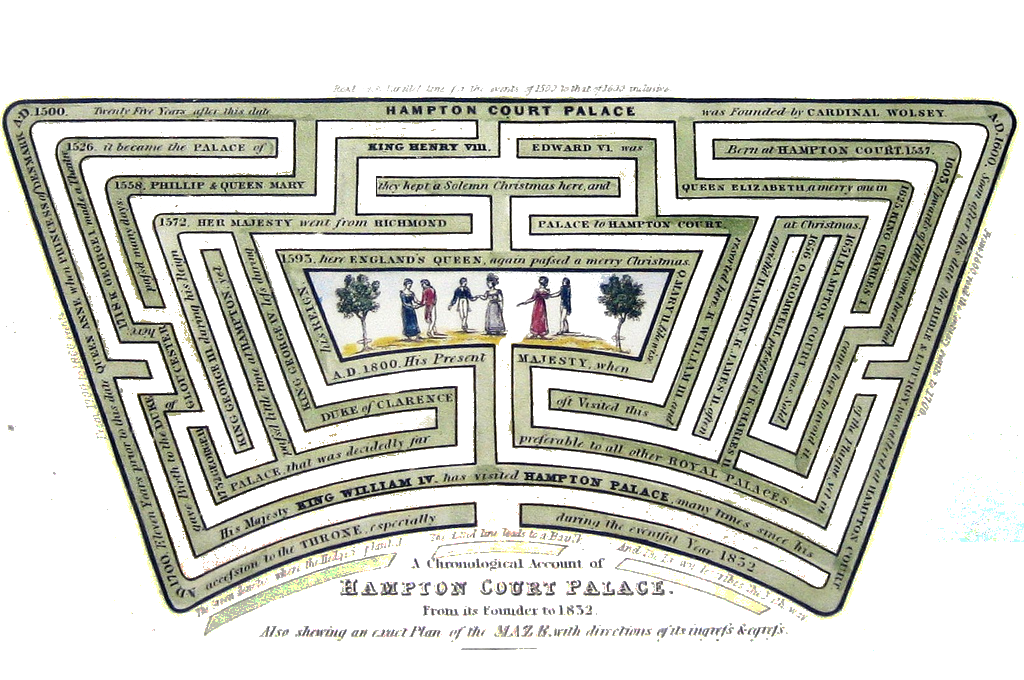
\includegraphics[height=80mm]{assets/hampton1.png}
\end{frame}

\begin{frame}
  \centering
  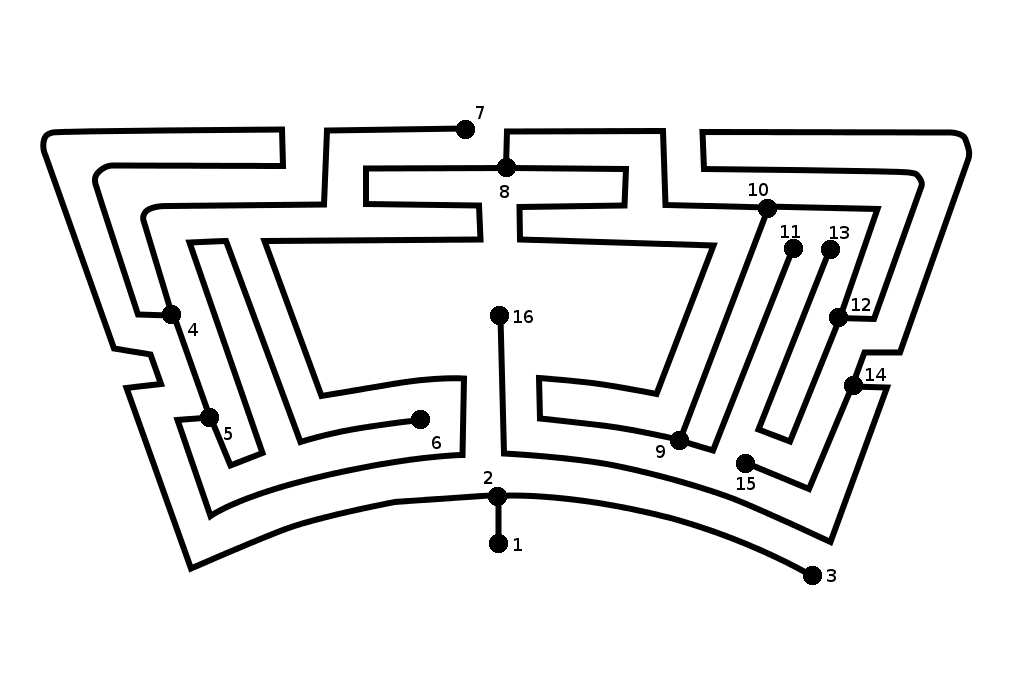
\includegraphics[height=80mm]{assets/hampton2.png}
\end{frame}

\begin{frame}
  \centering
  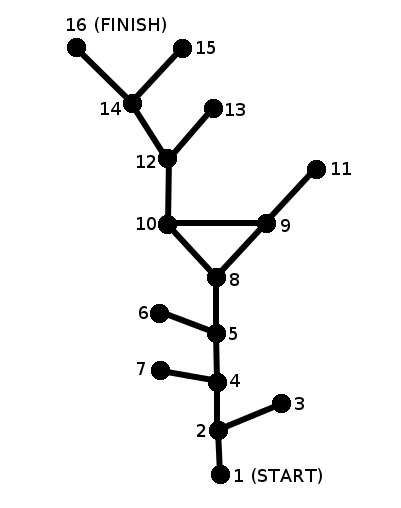
\includegraphics[height=80mm]{assets/hampton3.png}
\end{frame}

\begin{frame}
  \centering
  
\includegraphics[width=80mm]{assets/maze.pdf}
\end{frame}

\begin{frame}
  \centering
  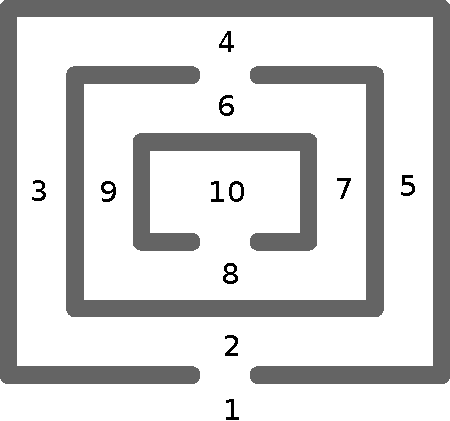
\includegraphics[width=80mm]{assets/maze-b1-crop.pdf}
\end{frame}

\begin{frame}
  \centering
  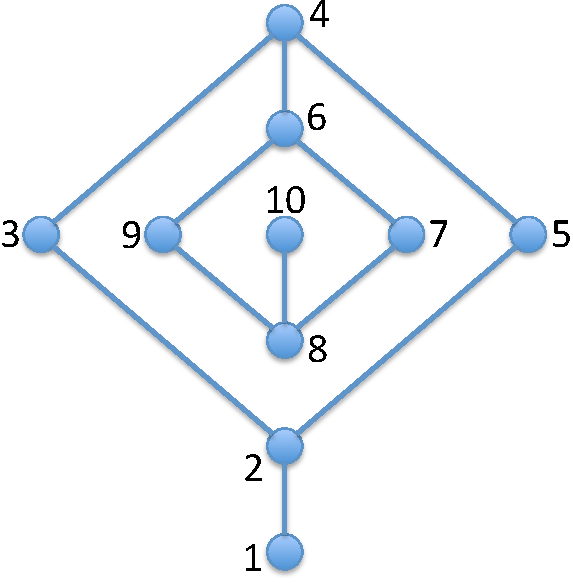
\includegraphics[height=80mm]{assets/maze-b2-crop.pdf}
\end{frame}

\begin{frame}
  \centering
  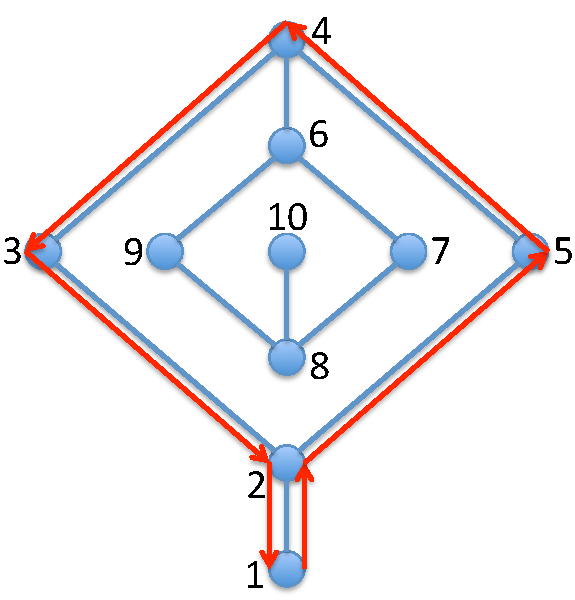
\includegraphics[width=70mm]{assets/maze-b3-crop.pdf}
\end{frame}

\begin{frame}
  \centering
  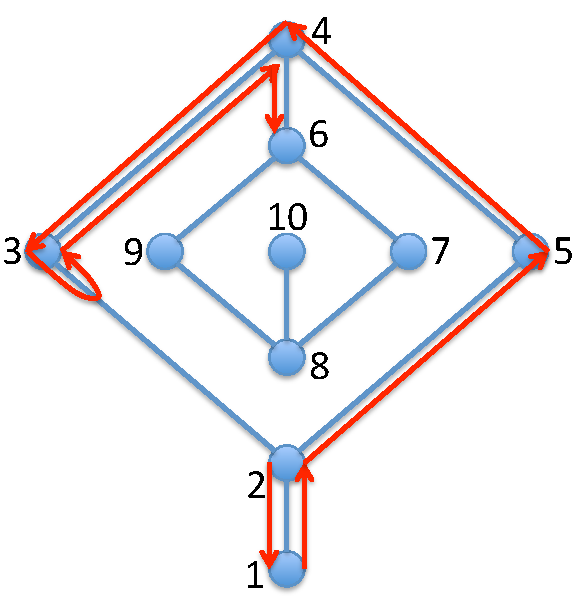
\includegraphics[width=70mm]{assets/maze-b4-crop.pdf}
\end{frame}

\begin{frame}
  \centering
  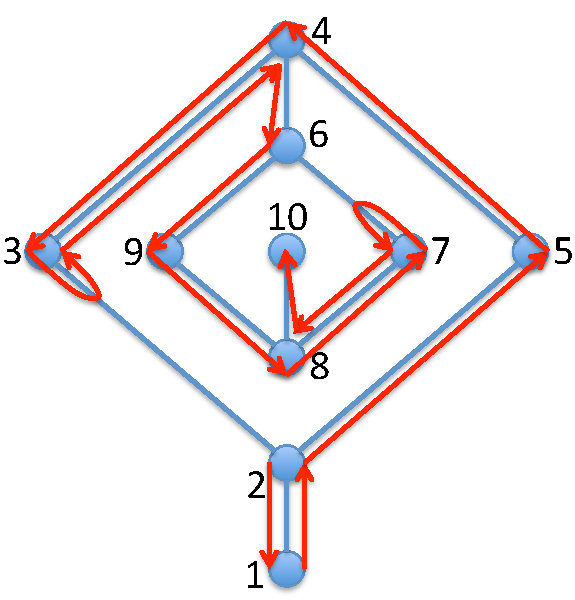
\includegraphics[width=70mm]{assets/maze-b5-crop.pdf}
\end{frame}

\begin{frame}
  \frametitle{Noughts and Crosses}
  \begin{center}
    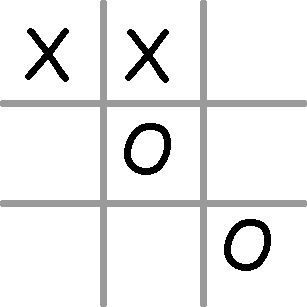
\includegraphics[width=0.3\textwidth]{assets/oxo-board1.pdf}
    \end{center}

  $9\times8\times7\times6\times5\times4\times3\times2\times1$ or 9! = 362,880 moves

  Many games finish before board is full, so 255,168 possible different games.

  (Actually, less due to symmetry, but I'm going to ignore that.)

  Adding one extra rule, \textit{always win if you can}, reduces this to 52,592.
\end{frame}
\begin{frame}
  Consider a position close to the end of the game:

  \begin{center}
  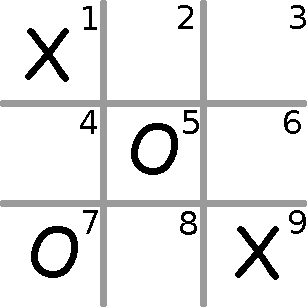
\includegraphics[width=0.3\textwidth]{assets/oxo-board3.pdf}
      \end{center}

  We're playing {\sf X} and we started, so it's our go.  Where should we play?
\end{frame}

\begin{frame}
  How about position 2?
  \begin{center}
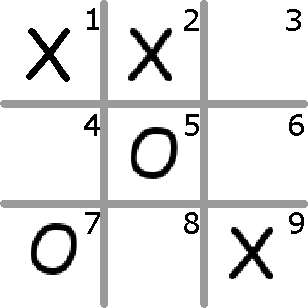
\includegraphics[width=0.3\textwidth]{assets/oxo-board3b.pdf}
\end{center}
\end{frame}

\begin{frame}
  O wins
\begin{center}
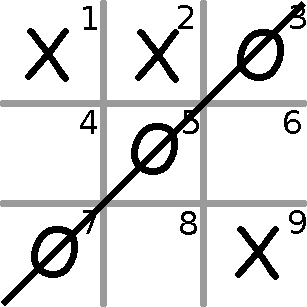
\includegraphics[width=0.3\textwidth]{assets/oxo-board4.pdf}
\end{center}
\end{frame}

\begin{frame}
  Backtrack, and mark square 2 as ``lose''
\begin{center}
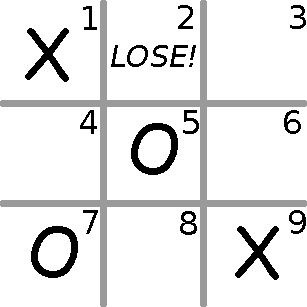
\includegraphics[width=0.3\textwidth]{assets/oxo-board5.pdf}
\end{center}
\end{frame}

\begin{frame}
  The same thing happens when we explore squares 4, 6, and 8, so those get marked as Lose too.
  \begin{center}
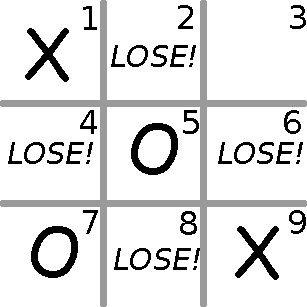
\includegraphics[width=0.3\textwidth]{assets/oxo-board6.pdf}
\end{center}
\end{frame}

\begin{frame}
  How about square 3?
  \begin{center}
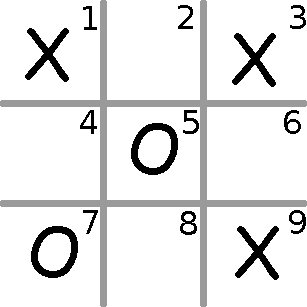
\includegraphics[width=0.3\textwidth]{assets/oxo-board7.pdf}
\end{center}
\end{frame}
\begin{frame}
  
    Now we have to try all of O's possible moves.

    First try O at square 2.
  \begin{center}
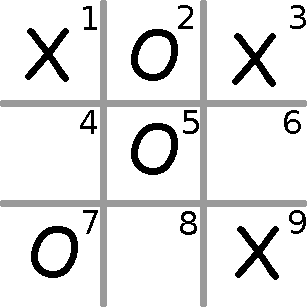
\includegraphics[width=0.3\textwidth]{assets/oxo-board8.pdf}
  \end{center}

  We'll play at 6 to win.  But can O play elsewhere to force a win?
\end{frame}
\begin{frame}
    Next try O at square 4.

    \begin{center}
\hspace{0.25in}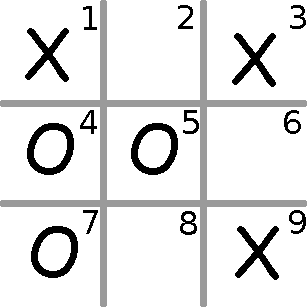
\includegraphics[width=0.3\textwidth]{assets/oxo-board9.pdf}
\end{center}

    We'll play at 6 to win.  But can O play elsewhere to force a win?
\end{frame}
\begin{frame}
    Next try O at square 6.
  
  \begin{center}
\hspace{0.25in}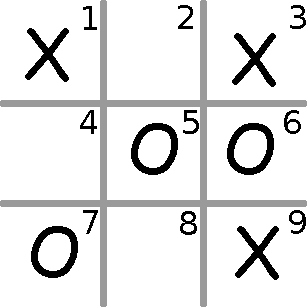
\includegraphics[width=0.3\textwidth]{assets/oxo-board10.pdf}
\end{center}

    We'll play at 2 to win.  But can O play elsewhere to force a win?
\end{frame}

\begin{frame}
    Finally try O at square 8.
  \begin{center}
\hspace{0.25in}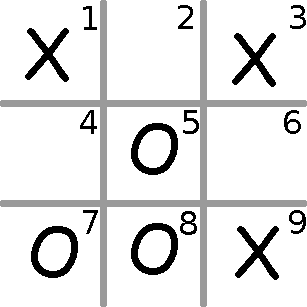
\includegraphics[width=0.3\textwidth]{assets/oxo-board11.pdf}
\end{center}
    We'll play at 2 or 6 to win.  O has no winning moves.
\end{frame}

\begin{frame}
    Backtrack and mark square 3 as ``win''.

    \begin{center}
\hspace{0.25in}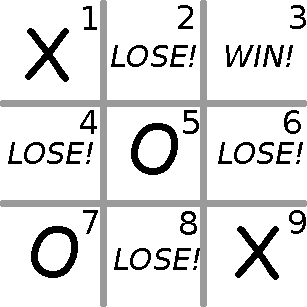
\includegraphics[width=0.3\textwidth]{assets/oxo-board12.pdf}
\end{center}
\end{frame}

%\begin{frame}
%%   \begin{center}
%% 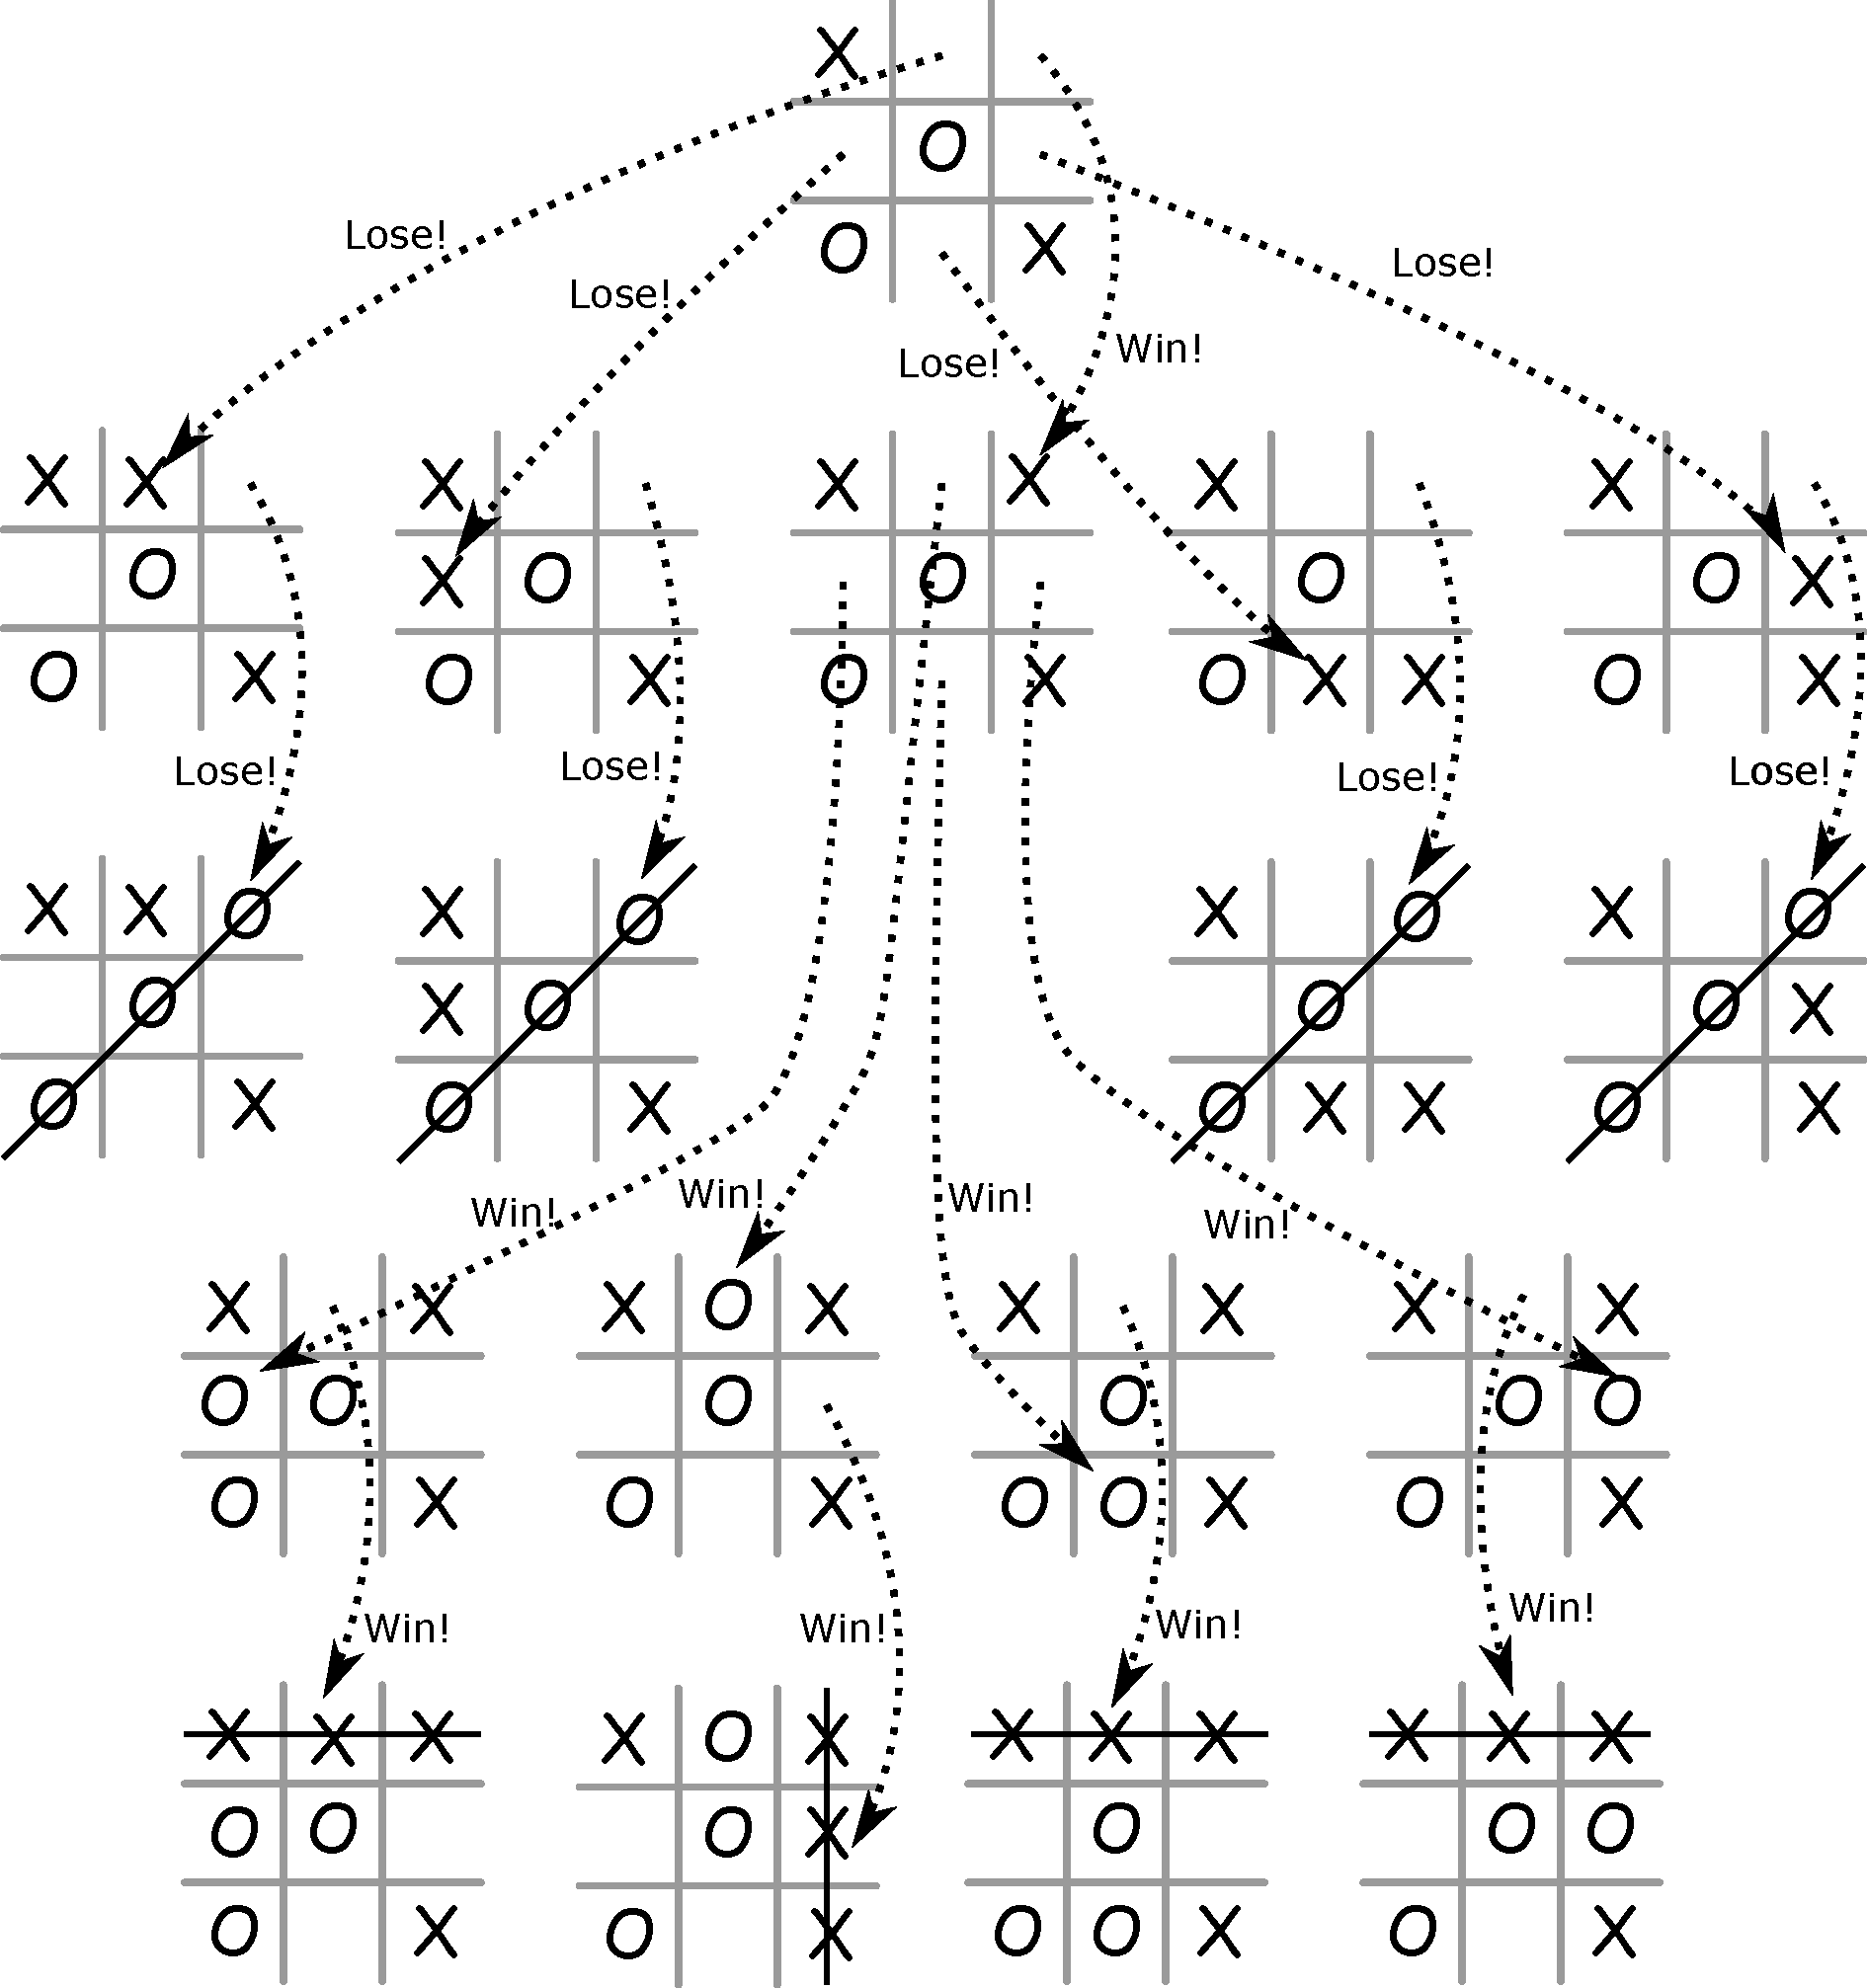
\includegraphics[height=80mm]{assets/oxo-board-full2.pdf}
%% \end{center}
%% \end{frame}
%% \begin{frame}
  
%%   \begin{center}
%% 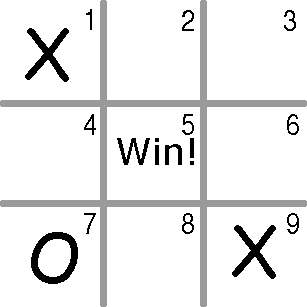
\includegraphics[width=0.3\textwidth]{assets/oxo-board15.pdf}
%% \end{center}
%% \end{frame}
%% \begin{frame}
  
%%   \begin{center}
%% 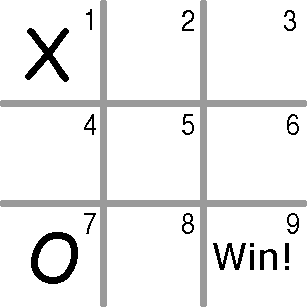
\includegraphics[width=0.3\textwidth]{assets/oxo-board16.pdf}
%% \end{center}
%% \end{frame}

%% \begin{frame}
%%   \begin{center}
%% 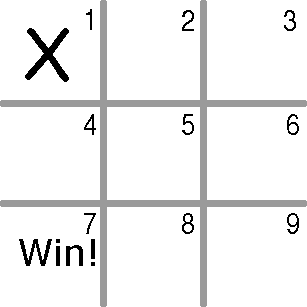
\includegraphics[width=0.3\textwidth]{assets/oxo-board17.pdf}
%% \end{center}
%% \end{frame}

  \begin{frame}
    If we do this search from move 1, we get:
  \begin{center}
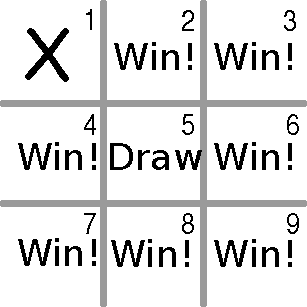
\includegraphics[width=0.3\textwidth]{assets/oxo-board18.pdf}
\end{center}
\end{frame}

  \begin{frame}
  \begin{center}
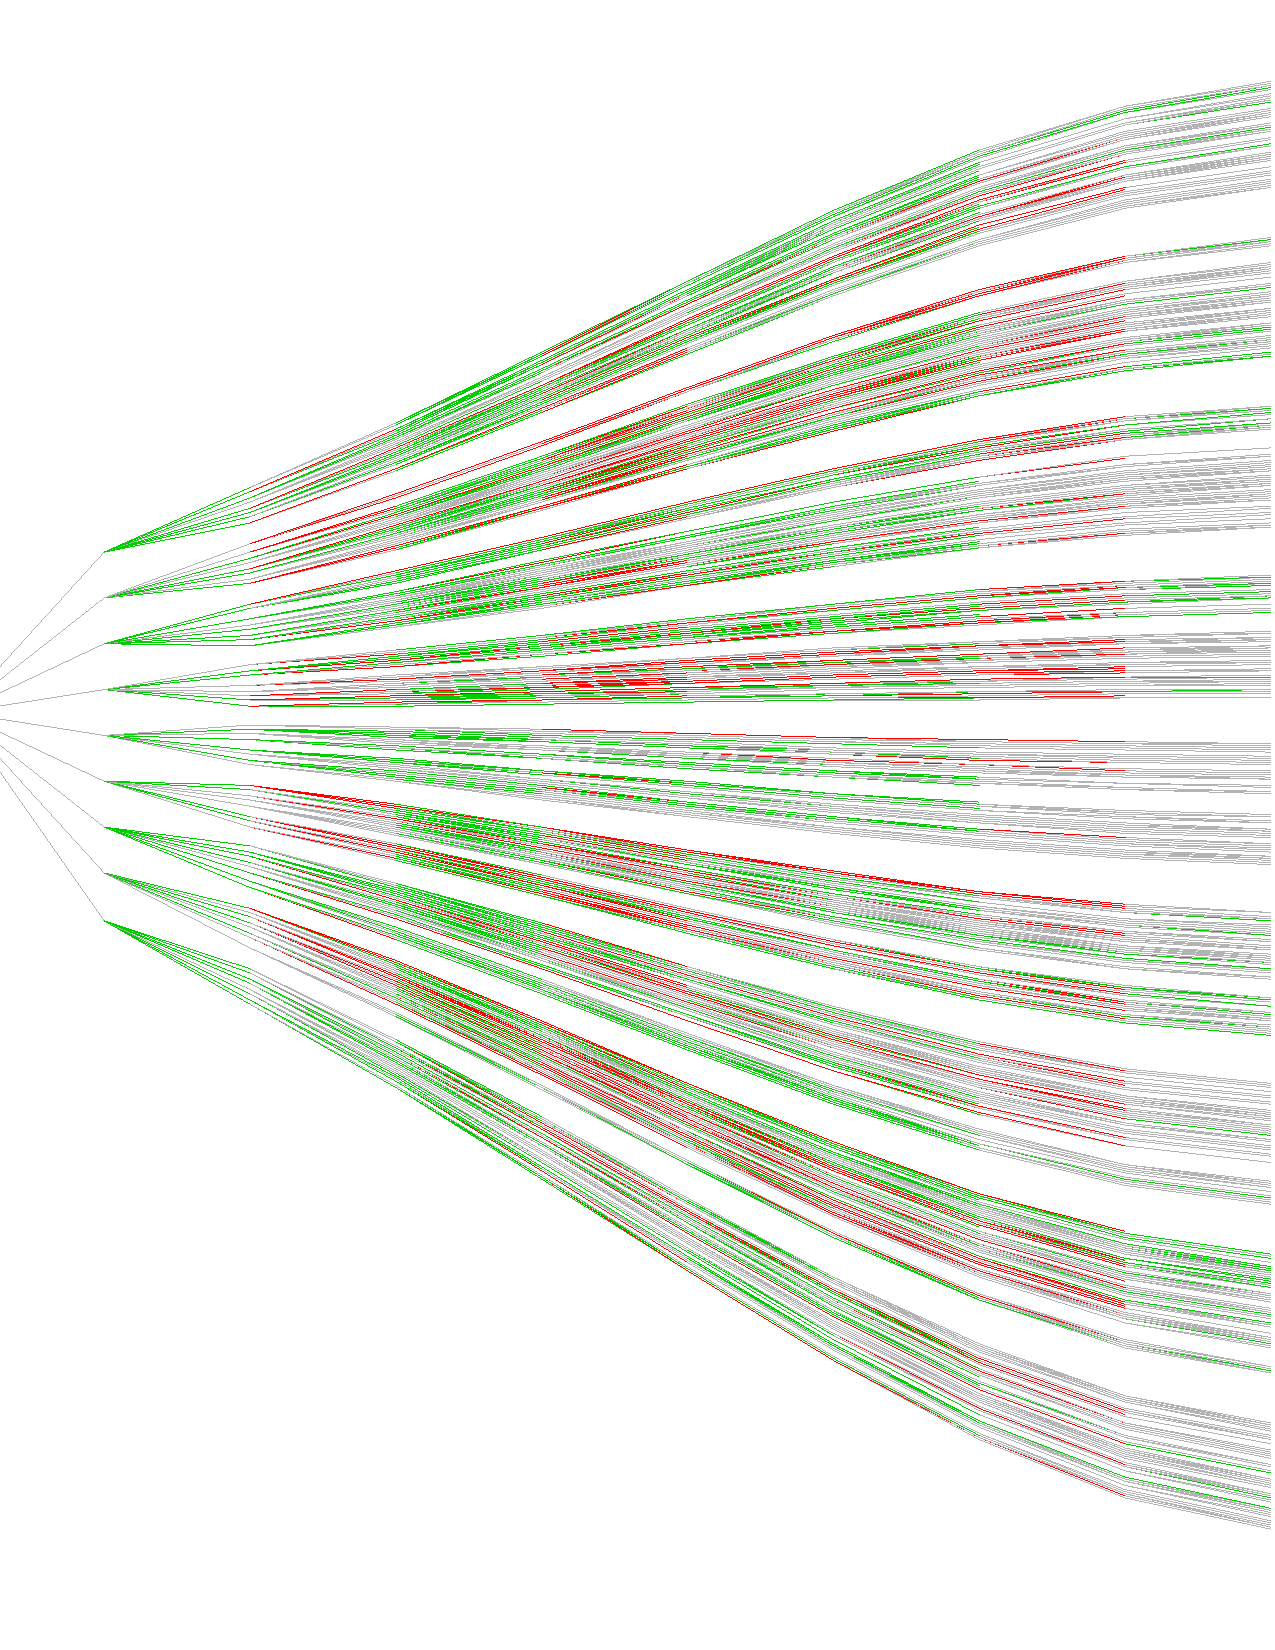
\includegraphics[height=80mm]{assets/oxo-full-tree-color.pdf}
\end{center}
\end{frame}

  \begin{frame}
    Wargames, 1983
  \begin{center}
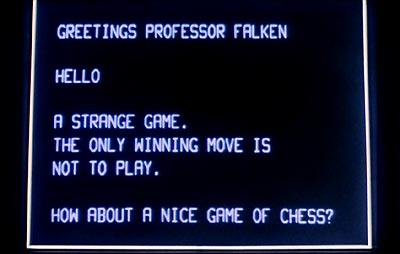
\includegraphics[width=90mm]{assets/wargames_chess_request.jpg}
\end{center}
\end{frame}

\bibliographystyle{alpha}
\nobibliography{references}

\end{document}
